\chapter{Evaluation}
\label{chapter:evaluation}

We need some sort of tool to measure the ``goodness'' of the 
clustering. As we work with text data the dimesionality increases 
quite high and projecting data down to 2 or 3 dimensions for 
visualization is not a simple task. (We come back to visualization 
later though.)
So we have to resort to measurements derived from the 
resulting clustering itself. If we knew some underlying ground 
truth behind our clustering problem we could validate our result 
against it. But as mentioned earlier, even defining what actually 
are the current fields of science depends on who you ask and for 
what purpose the definition is needed. So the the ground truth 
here is only one measure for our results.
In the lack of ground truth we can use some ``internal'' goodness 
measure for the resulting clustering. These kind of measures 
basically try to infer how dense the clusters are compared to how 
sparse the inter-cluster space is and how well the clusters are 
separated from each other.
One such measure to estimate the ``goodness'' of a clustering is 
silhouettes. Silhouettes use average proximities which are know 
to work best with clear, compact and spherical clusters 
\cite{rousseeuw_silhouettes:_1987}. Silhouette value for an item 
is defined as:

Silhoutte values for 6000 publications clustered with 
agglomerative clustering with Ward's method, number of clusters 
64, are seen in Figure~\ref{fig:silh01}.
\begin{figure}[ht]
  \begin{center}    
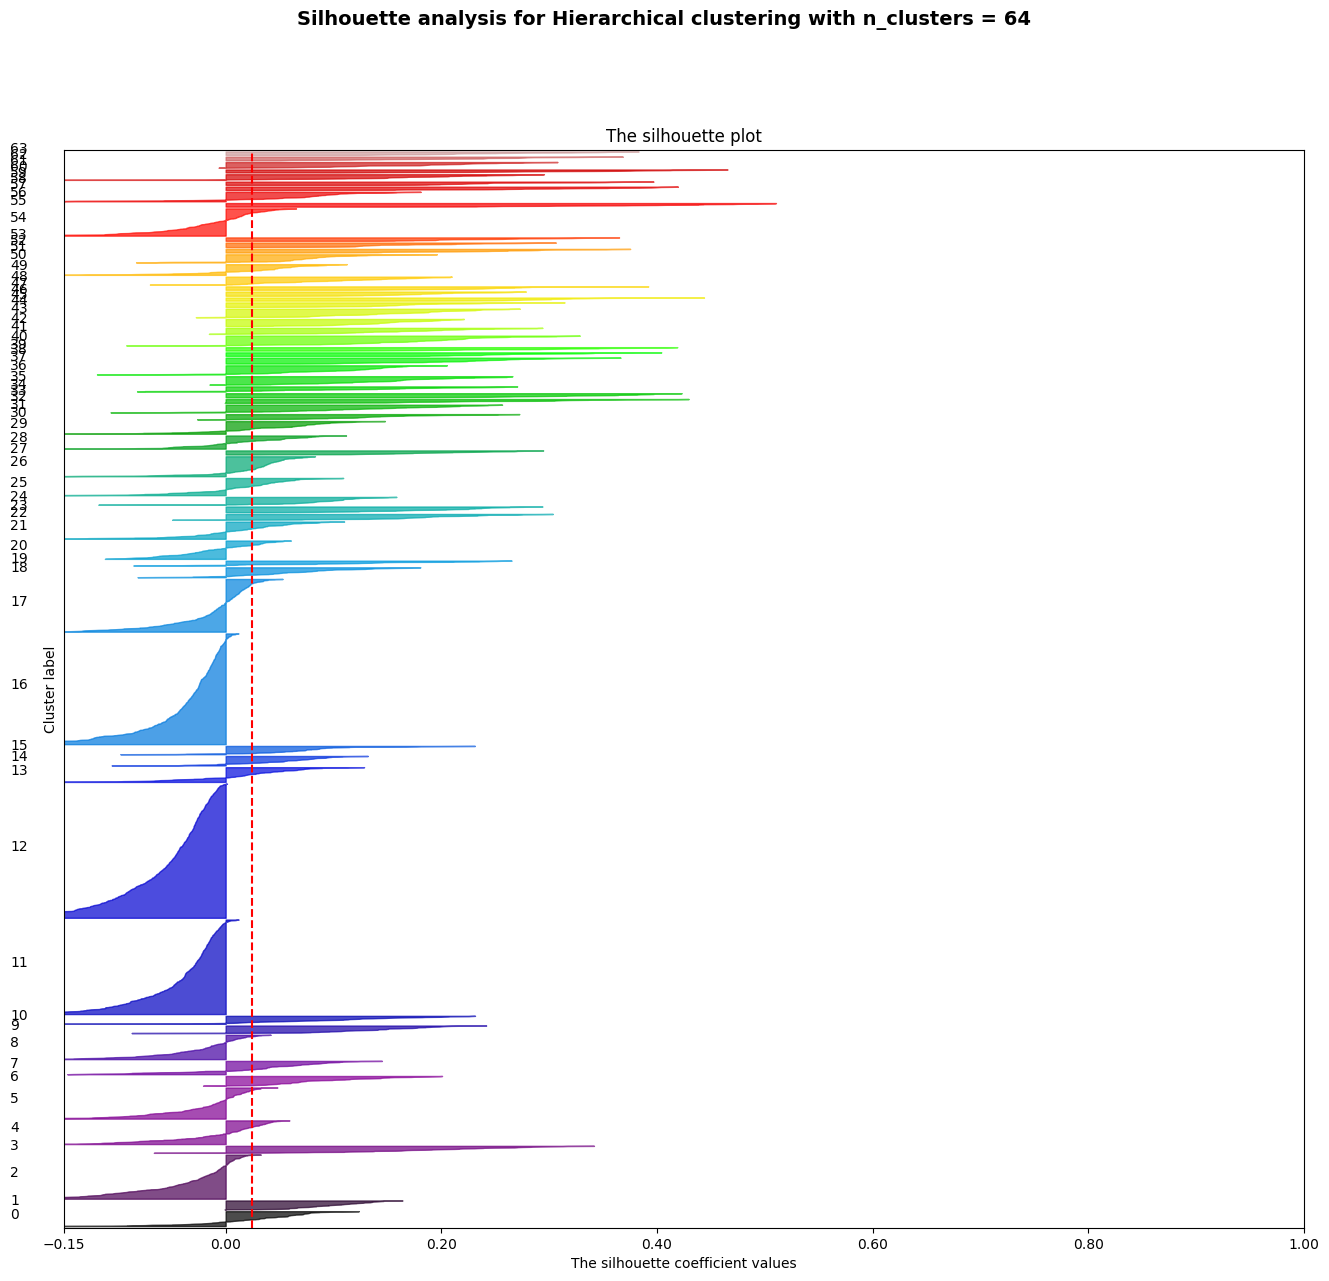
\includegraphics[width=13cm]{images/6000-64-400-Hierarchical-silhouette-plot.png}
    \caption{Silhoutte values of 6000 items clustered with 
    agglomerative clustering with Wrad's method, 64 clusters, 
    LSA with 400 components. Each pixel row corresponds to a 
    Silhouette value of an item, adjacent rows separated by gap 
    corresponds to a cluster.
    Dashed line is the average.}
    \label{fig:silh01}
  \end{center}
\end{figure}

Other measure is Calinski-Harabaz index. Clustering should be 
optimal when Calinski-Harabaz index reaches its maximum value. 
\cite{}

When evaluating the results, Silhouette Coefficient might not be
the best option. Find out why. V-measure or Adjusted Rand Index
might be better options \cite{noauthor_clustering_nodate}.

We could evaluate our clustering by creating an evaluation set with
hand labeled or verified fields of science. Then we could use
regular measurement methods that rely on having ground truth 
available. Of course the ground truth would be our own subjective 
definition. \fixme{I am actually about to manually check some 500
documents belonging to two quite similar one more different 
discipline. Based on that ground truth I will calculate precision
and recall for a clustering.}

Different metrics to evaluate clustering include (from 
scikit-learn) Adjusted Rand Index, Mutual Information scrores 
(NMI, AMI), homogenity, completness, V-measure, Fowlkes-Mallows 
scores, Silhouette Coefficient, Calinski-Harabaz Index, (from 
sources) 

